\documentclass{beamer}

\usepackage{beamerthemeCVC}

\usepackage{graphicx}

\setbeamertemplate{caption}[numbered]

\usepackage{xmpmulti}

%% PRESENTATION CONFIGURATION PARAMETERS %%%%%%%%%%%%%%%%%%%%%%%%%%%%%%%%%%%%%%%
%  \titlebackgroundfile{images/template_title}
%  \framebackgroundfile{images/template_frame_v05}


%\definecolor{vermell}{HTML}{8C2423}
\definecolor{vermell}{HTML}{000066}
\definecolor{gris}{HTML}{4C4C4C}

% http://latexcolor.com/
\definecolor{anti-flashwhite}{rgb}{0.95, 0.95, 0.96}
\definecolor{palesilver}{rgb}{0.79, 0.75, 0.73}



\usefonttheme[onlymath]{serif}


%Font
% \usefonttheme{professionalfonts}
% \usepackage[utf8]{inputenc}
% \usefonttheme{default}

% \usefonttheme[onlymath]{serif}
% % http://tex.stackexchange.com/questions/34265/how-to-get-beamer-math-to-look-like-article-math



% http://tex.stackexchange.com/questions/183052/what-are-all-the-possible-first-arguments-to-setbeamerfont/183053#183053

\setbeamercolor{title in head/foot}{fg=vermell}


\setbeamercolor{author in head/foot}{fg=palesilver}
%
\setbeamercolor{framenumber in head/foot}{fg=vermell}



\setbeamercolor{section in head/foot}{fg=vermell}
\setbeamercolor{normal text}{fg=gris}
%\setbeamercolor{frametitle}{fg=vermell}
\setbeamercolor{frametitle}{fg=blue!20!black}

\setbeamerfont{block title}{size={}}
\setbeamerfont{author}{size=\footnotesize}
\setbeamerfont{date}{size=\footnotesize}

\setbeamerfont{footline}{size=\fontsize{3}{11}\selectfont}


\setbeamertemplate{itemize item}[circle]
\setbeamertemplate{itemize subitem}[circle]
\setbeamertemplate{itemize subsubitem}[circle]
\setbeamertemplate{itemize subsubsubitem}[circle]
\setbeamercolor{itemize item}{fg=vermell}
\setbeamercolor{itemize subitem}{fg=vermell}
\setbeamercolor{itemize subsubitem}{fg=vermell}
\setbeamercolor{itemize subsubsubitem}{fg=vermell}
\setbeamercolor{enumerate item}{fg=vermell}
\setbeamercolor{enumerate subitem}{fg=vermell}
\setbeamercolor{enumerate subsubitem}{fg=vermell}
\setbeamercolor{enumerate subsubsubitem}{fg=vermell}
\setbeamercolor{alerted text}{fg=vermell}
\setbeamerfont{alerted text}{series=\bfseries}
% This command makes that acrobat reader doesn't changes the colors of the slide
% when there are figures with transparencies.
\pdfpageattr {/Group << /S /Transparency /I true /CS /DeviceRGB>>}



%\setbeamerfont{bibliography entry author}{series=\bfseries}
% \setbeamerfont{bibliography entry title}{series=\bfseries}
% \setbeamerfont{bibliography item}{series=\bfseries}

\setbeamerfont{bibliography item}{size=\scriptsize}
\setbeamerfont{bibliography entry author}{size=\scriptsize}
\setbeamerfont{bibliography entry title}{size=\scriptsize}
\setbeamerfont{bibliography entry location}{size=\scriptsize}
\setbeamerfont{bibliography entry note}{size=\scriptsize}

% \usepackage{hyperref}
% \hypersetup{colorlinks=true, linkcolor=blue}
% \renewcommand*{\bibfont}{\scriptsize}

\graphicspath{{images/}}






%%%%%%%%%%%%%%%%%%%%%%%%%%%%%%%%%%%%%%%%%%%%%%%%%%%%%%%%%%%%%%%%%%%%%%%%%%%%%%%%

%      + Short title.               + Title which appears in the cover.
%      v                            v
%\title[Beamer presentation example]{Nonlinear Dynamics Approach to Human Activity Recognition Using Inertial Sensors}
\vspace{5mm}
\title[Analysis of the Movement Variability in Dance Activities Using Wearable Sensors]
{Analysis of the Movement Variability in Dance Activities Using Wearable Sensors}
%       + Short author names which appear in the slides.
%       v
\author[Miguel Xochicale]
{   % Author names which appear in the cover page.
    %Perez-Xochicale Miguel Angel
    Miguel Xochicale\inst{1}, Chris Baber\inst{1} and Mourad Oussalah\inst{2}
}
%          + Short affiliation which appears in the slides.
%          v
\institute[CVC-IIIA]
{   % Affiliation information which appears in the cover page.

      \vspace{5mm}
    \begin{tabular}{c}
    \inst{1} School of Electronic, Electrical and System Engineering, University of Birmingham, U.K. \\
    \inst{2} Center for Ubiquitous Computing, University of Oulu, Finland
    \end{tabular}
}
%     + Short acronym of the conference or date of the presentation.
%     v
\date[DEMO-2013]
{   % Conference name which appears in the cover page.
      \vspace{5mm}
     The 2nd International Symposium on Wearable Robotics \\
     La Granja de San Idelfonso, Segovia, Spain \\
     18-21 October 2016
}





\newif\iflattersubsect

\AtBeginSection[] {
    \begin{frame}<beamer>
    \frametitle{Outline} %
    \tableofcontents[currentsection]
    \end{frame}
    \lattersubsectfalse
}

\AtBeginSubsection[] {
    \iflattersubsect
    \begin{frame}<beamer>
    \frametitle{Outline} %
    \tableofcontents[currentsubsection]
    \end{frame}
    \fi
    \lattersubsecttrue
}




\begin{document}
% Creates the cover page.
\frame{\titlepage}





\begin{frame}
\frametitle{Outline}
\tableofcontents
\end{frame}




%+++++++++++++++++++++++++++++++++++++++++++++++++++
%+++++++++++++++++++++++++++++++++++++++++++++++++++
\section{I. Introduction}








%%+++++++++++++++++++++++++++++++++++++++++++++++++++
\begin{frame}
\frametitle{Movement Variability}

Movement Variability is an inherent feature that occurs not only within individual
but also between individual systems of movement  \textcolor{red}{\textbf{ \cite{newell1993variability}   }}.

\end{frame}


 %%+++++++++++++++++++++++++++++++++++++++++++++++++++
\begin{frame}
\frametitle{Inter-trial Movement Variability}

\textcolor{red}{\textbf{  \cite{Preatoni2013}   }} mentioned that
 inter-trial variability is a combination of
\begin{itemize}
    \item noise in the neuro-musculo-skeletal system, and
    \item functional changes that might be associated with the exploration of different
stragies to find the most effective one among many available.
\end{itemize}



\end{frame}




 % %+++++++++++++++++++++++++++++++++++++++++++++++++++
\begin{frame}
  \frametitle{Motor Variability is not noise}


  \begin{figure}
 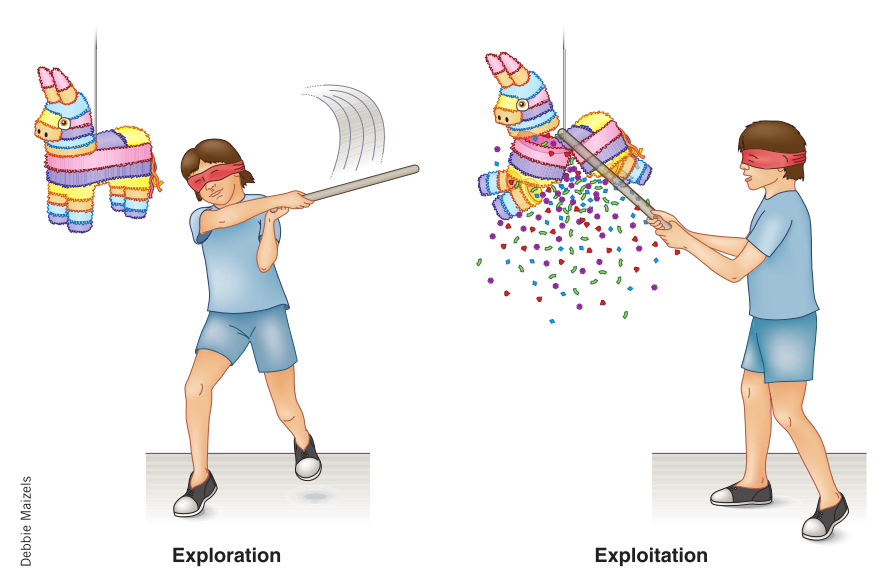
\includegraphics[width=0.7\textwidth]{herzfelt2014_fig1}
\centering
\caption{Find the pi\~nata \textcolor{red}{\textbf{  \cite{Herzfeld2014}   }}.}
 \end{figure}



\end{frame}





%%+++++++++++++++++++++++++++++++++++++++++++++++++++
\begin{frame}
\frametitle{Nonlinear Dynamics to  Movement Variability}


According to \textcolor{red}{\textbf{  \cite{Preatoni2013}   }},
some nonlinear dynamics tools to explore the nature of movement variability
and its relationship with skills development are:
\begin{itemize}
    \item Phase Space Representation.
    \item Lyapunov Exponent.
\end{itemize}


\end{frame}




%+++++++++++++++++++++++++++++++++++++++++++++++++++
%+++++++++++++++++++++++++++++++++++++++++++++++++++
\section{II. Methods}







\subsection{A. Time-delay embedding}


% \frame{\tableofcontents[currentsection, currentsubsection]} %new code





%+++++++++++++++++++++++++++++++++++++++++++++++++++
\begin{frame}
\frametitle{Time-delay embedding theorem}
\vspace{-0.7cm}


For a given discrete time-series $x(n) = [x(1) , x(2), \dots, x(N)]$,
a reconstructed state space can be created by
\begin{eqnarray*}
\overline{x}(n) = [ x(n), x(n - \tau), x(n-2\tau), \dots , x (n-(m-1)\tau) ]
\end{eqnarray*}
which creates a concatenated column-wise matrix of the time-delay versions of the original signal:
\begin{equation}
  \resizebox{\textwidth}{!}{$\displaystyle
  \mathbf{X}
    = \begin{pmatrix} \nonumber
      x(1) & x(1 - \tau) & x(1-2\tau) & \dots & x (1-(m-1)\tau) \\
      x(2) & x(2 - \tau) & x(2-2\tau) & \dots & x (2-(m-1)\tau) \\
      \vdots &  &  & \ddots & \vdots \\
      x(N) & x(N - \tau) & x(N-2\tau) & \dots & x (N-(m-1)\tau) \\
      \end{pmatrix}
     $}
\end{equation}



where $m$ is the \textbf{ embedding dimension}  and  $\tau$ is the \textbf{ embedding delay}
\textcolor{red}{\textbf{  \cite{Takens1981} }}.
False Nearest Neighborhood and Mutual Information algorithms are used to compute
the optimal value of $m$ and $\tau$.

\end{frame}
%---------------------------------------------------






%+++++++++++++++++++++++++++++++++++++++++++++++++++
%+++++++++++++++++++++++++++++++++++++++++++++++++++
\subsection{B. Framework of the experiment}



%+++++++++++++++++++++++++++++++++++++++++++++++++++
\begin{frame}
\frametitle{Percentage Of Variance}
\vspace{-0.7cm}

The Percentage of variance (POV) is obtained by using the PCA.
\begin{figure}[!htb]
\centering
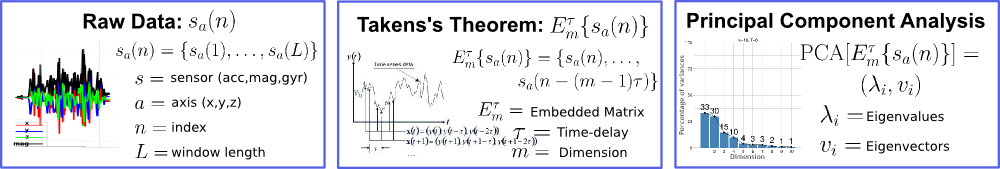
\includegraphics[width=1\textwidth]{method_diagram03}
\caption[PA]{Percentage of Cummulative Energy}
 \label{fig:sn}
\end{figure}

\vspace{-0.7cm}

\begin{figure}[!htb]
\centering
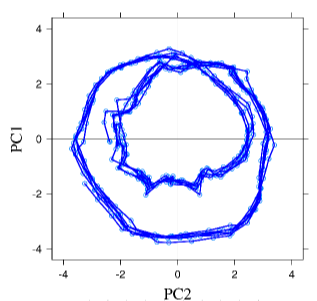
\includegraphics[width=.35\textwidth]{rss00}
\caption[PA]{Reconstructed State Space}
 \label{fig:sn}
\end{figure}


\end{frame}
%---------------------------------------------------









%+++++++++++++++++++++++++++++++++++++++++++++++++++
%+++++++++++++++++++++++++++++++++++++++++++++++++++
\subsection{C. Participants}









%+++++++++++++++++++++++++++++++++++++++++++++++++++
\begin{frame}
\frametitle{Participants}
\vspace{-0.7cm}

Thirteen participants with different years of experience
in dancing were invited to dance basic salsa steps:

\begin{itemize}
    \item eleven (4 female, 7 male) novice dancers (none or less than two months of experience);
    \item one male intermediate (4 years of experience); and,
    \item one male expert (14 years of experience)
\end{itemize}



\end{frame}
%---------------------------------------------------


%+++++++++++++++++++++++++++++++++++++++++++++++++++
%+++++++++++++++++++++++++++++++++++++++++++++++++++
\subsection{D. Data Collection}

%+++++++++++++++++++++++++++++++++++++++++++++++++++
\begin{frame}
\frametitle{Razor 9DOF IMU}
\vspace{-0.7cm}

Data collection from triaxial accelerometer, gyroscope and magnetometer sensors
at a sampling rate of 50Hz for 20 seconds.

\begin{figure}[!htb]
\centering
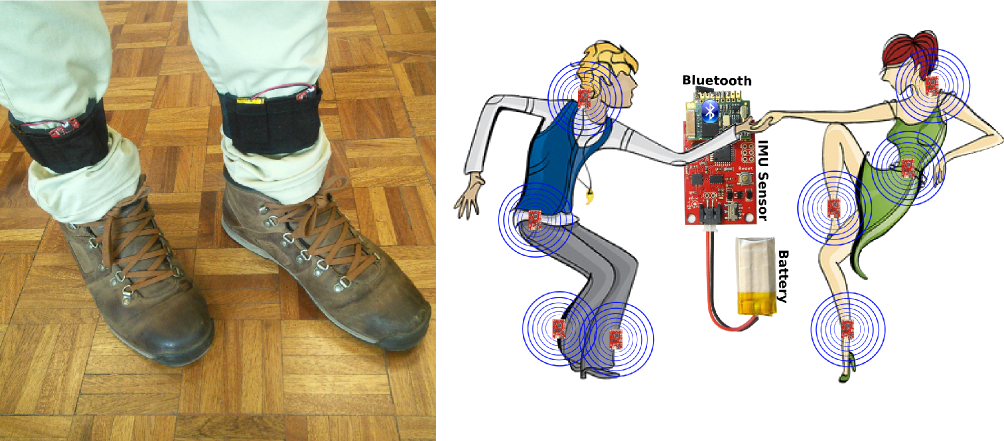
\includegraphics[width=0.7\textwidth]{datacollection01}
\caption[PA]{IMU sensors mounted on left and right ankle}

\label{fig:sn}
\end{figure}



\end{frame}
%---------------------------------------------------







%+++++++++++++++++++++++++++++++++++++++++++++++++++
%+++++++++++++++++++++++++++++++++++++++++++++++++++
\subsection{E. Experiment Design}

% \subsection{Design}





%+++++++++++++++++++++++++++++++++++++++++++++++++++
\begin{frame}
\frametitle{Basic Salsa Steps}
\vspace{-0.7cm}


\begin{figure}[!htb]
\centering
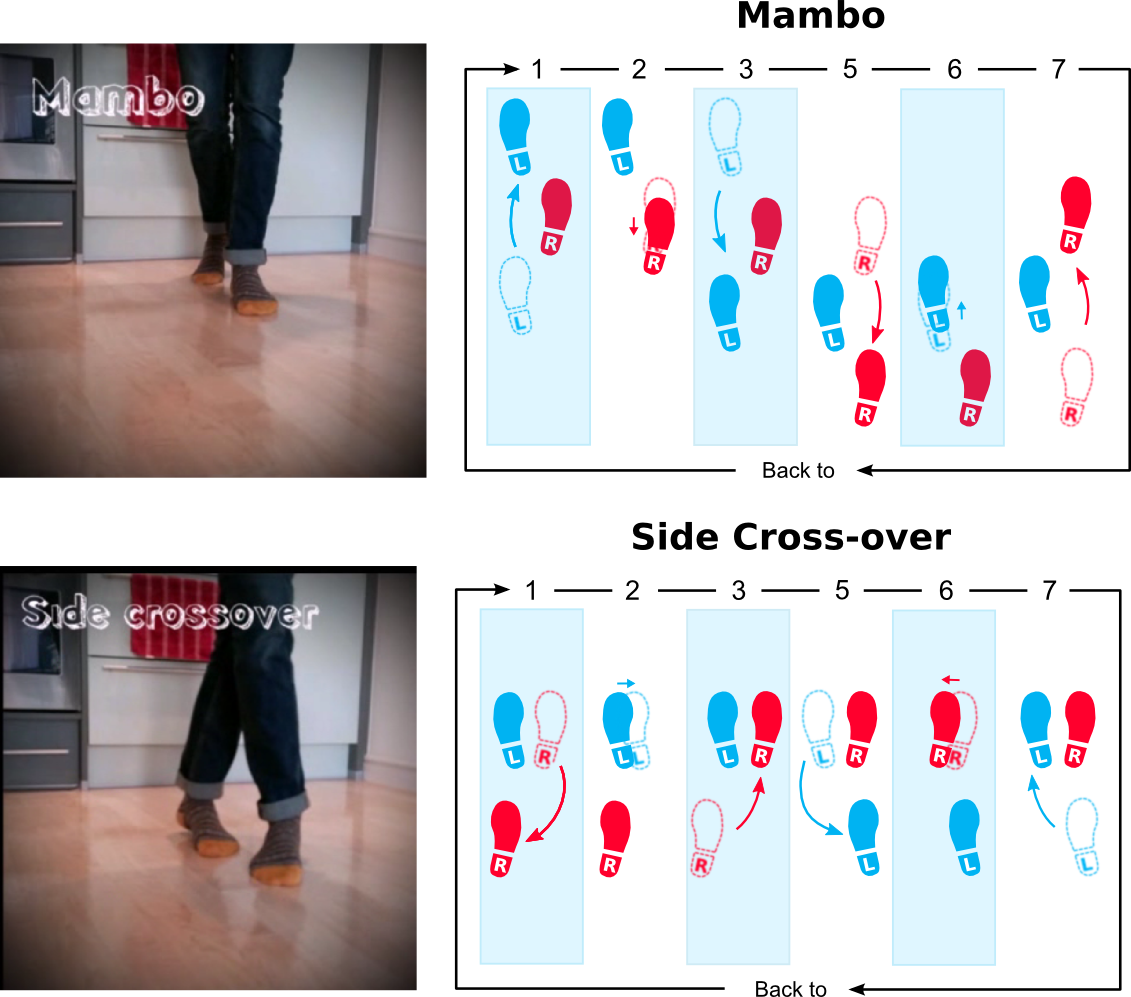
\includegraphics[width=0.7\textwidth]{steps00}
\caption[PA]{Mambo and Side Cross-over Steps}

\label{fig:sn}
\end{figure}



\end{frame}
%---------------------------------------------------


%




 %+++++++++++++++++++++++++++++++++++++++++++++++++++
%+++++++++++++++++++++++++++++++++++++++++++++++++++
\section{III. Results}






%+++++++++++++++++++++++++++++++++++++++++++++++++++
\begin{frame}
\frametitle{Visual levels of dexterity}
\vspace{-0.9cm}


\begin{figure}[!htb]
\centering
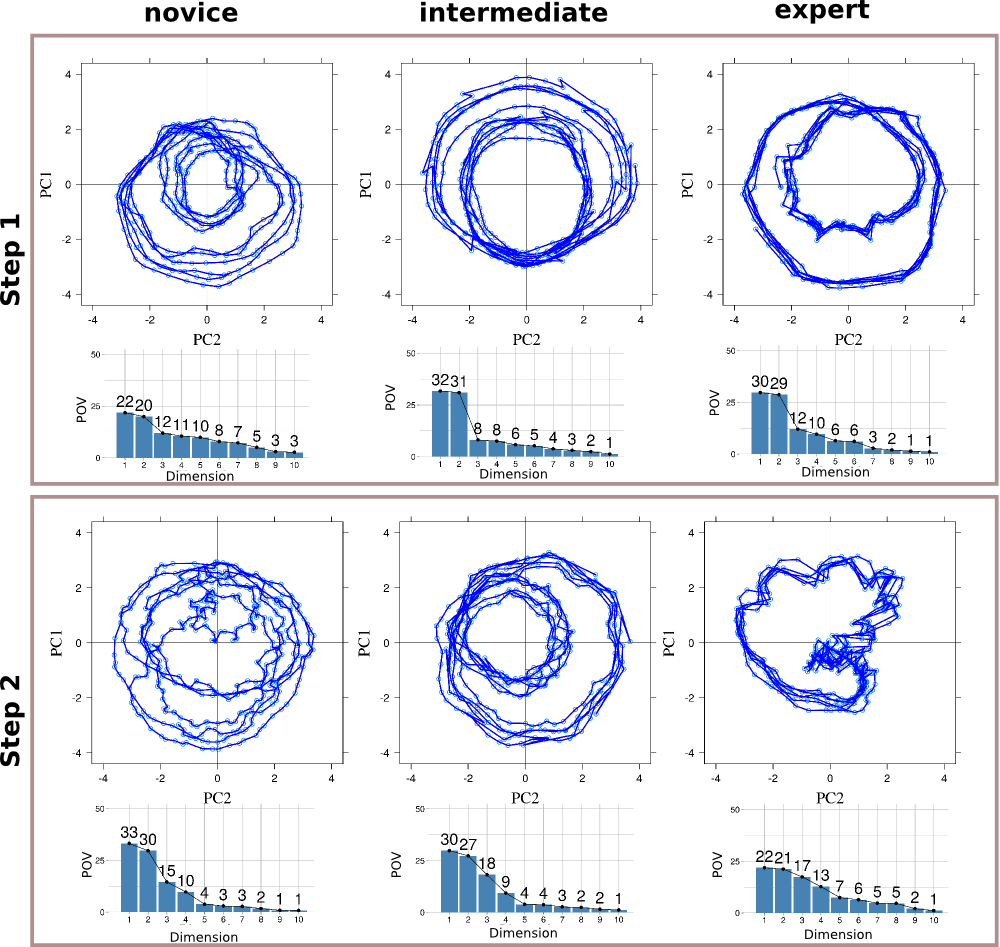
\includegraphics[width=0.7\textwidth]{main_figure_horizontal02}
\caption[PA]{2-D reconstructed state spaces and percentage of variance.}

\label{fig:sn}
\end{figure}



\end{frame}
%---------------------------------------------------






%+++++++++++++++++++++++++++++++++++++++++++++++++++
%+++++++++++++++++++++++++++++++++++++++++++++++++++
\section{IV. Conclusions and Future Work}






%+++++++++++++++++++++++++++++++++++++++++++++++++++
\begin{frame}
\frametitle{Conclusions}
\vspace{-0.7cm}

    \begin{itemize}
    \item (+) Visual difference between levels of skillfulness in simple dance activities
    using the time-delay embedding technique.
    \item (+) Extending the understanding of human movement variability.
    \end{itemize}

    \begin{itemize}
    \item (-) Time-delay embedding is subject to the embedded parameters ($m$ and $\tau$).
    \item (-) There is only one intermediate and one expert participant.

    \end{itemize}


\end{frame}
%---------------------------------------------------



%+++++++++++++++++++++++++++++++++++++++++++++++++++
\begin{frame}
\frametitle{Future Work}
\vspace{-0.7cm}

    \begin{itemize}
    \item Collect data from a wider range of individuals (gender and age) performing
    different simple movements with additional inertial sensors
    \item Undertake a wider review of nonlinear dynamics techniques.
    \item Explore the use of Hidden Markov Models and Deep Neural Networks
    for the automatic classification of the movement variability.
    \end{itemize}

    \begin{figure}[!htb]
    \centering
    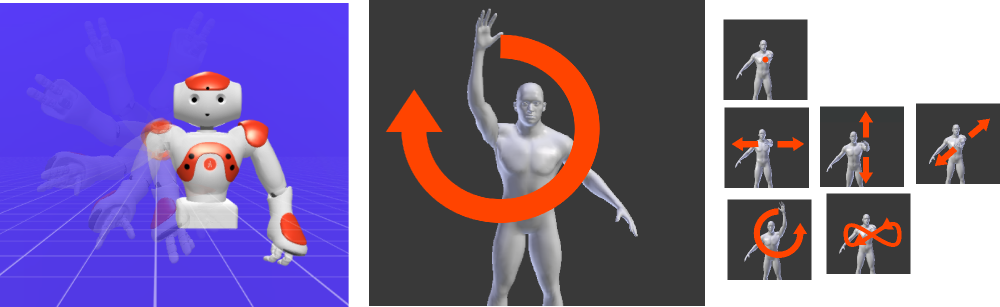
\includegraphics[width=0.7\textwidth]{future_work_00}
    \caption[PA]{Mirror Simple Movements Using NAO Robot}

    \label{fig:sn}
    \end{figure}


\end{frame}
%---------------------------------------------------



%+++++++++++++++++++++++++++++++++++++++++++++++++++
%
% % Creates the cover page.
%
%\frame{\titlepage}

\begin{frame}

\begin{center}
\textbf{GRACIAS}
\end{center}

\titlepage
\end{frame}
%---------------------------------------------------






%+++++++++++++++++++++++++++++++++++++++++++++++++++

\begin{frame}[fragile,allowframebreaks]{References}
  % In your presentation, remove `\nocite` here and
  % use `\cite` throughout the presentation.
  \nocite{*}

  \bibliographystyle{apalike}
  \bibliography{refslides}


%  \bibliography{D:/Gpai/Biblographies/library}
\end{frame}

%---------------------------------------------------



\end{document}
